% chktex-file 8
\section{Jadwal Pelaksanaan}

Berikut ini adalah beberapa tanggal capaian terkait pelaksaanaan pembuatan makalah ini:

\begin{enumerate}
  \item 18 Oktober 2021, pengumpulan studi literatur (Bab II).
  \item 15 November 2021, pengumpulan rencana topik tugas akhir (Bab I).
  \item 13 Desember 2021, pengumpulan proposal rancangan solusi (Bab III).
  \item 27 Desember 2021, pengumpulan buku makalah untuk tahap pertama atau proposal.
  \item 5-14 Januari 2022, rentang waktu pelaksanaan seminar tugas akhir pertama.
\end{enumerate}

Berikut adalah jangka waktu pengerjaan untuk makalah ini untuk tugas akhir ini sesuai dengan bagian metodologi:

\begin{table}[ht]
  \centering
  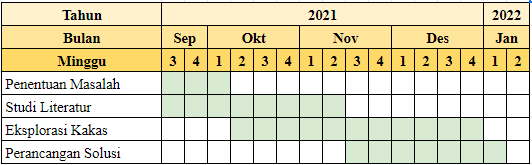
\includegraphics[width=0.8\textwidth]{01-jadwal.png}
  \caption{Jadwal Pelaksaaan Tugas Akhir}
\end{table}

% \begin{figure}
%   \centering
%   \begin{ganttchart}[
%     x unit=1mm,
%     inline,
%     milestone inline label node/.append style={left=5mm},
%     time slot format=isodate,
%     bar label font=\small
%     ]{2021-09-01}{2022-01-15}
%     \gantttitlecalendar{year, month=shortname} \\

%     % gantt tasks, milestones
%     \ganttbar{Topik}{2021-09-01}{2021-09-10} \\
%     \ganttbar{Bab II}{2021-09-14}{2021-10-18} \\
%     \ganttmilestone{Pengumpulan Bab II}{2021-10-18} \ganttnewline{}
%     \ganttbar{Bab I}{2021-10-18}{2021-11-15} \\
%     \ganttmilestone{Pengumpulan Bab I}{2021-11-15} \ganttnewline{}
%     \ganttbar{Bab III}{2021-11-15}{2021-12-13} \\
%     \ganttmilestone{Pengumpulan Bab III}{2021-12-13} \ganttnewline{}
%     \ganttbar{Buku TA I}{2021-12-13}{2021-12-27} \\
%     \ganttmilestone{Pengumpulan Buku TA I}{2021-12-27} \ganttnewline{}
%     \ganttmilestone{Sidang TA I}{2022-01-05} \ganttnewline{}
    
%     % links
%     \ganttlink{elem0}{elem1}
%     \ganttlink{elem1}{elem2}
%     \ganttlink{elem2}{elem3}
%     \ganttlink{elem3}{elem4}
%     \ganttlink{elem4}{elem5}
%     \ganttlink{elem5}{elem6}
%     \ganttlink{elem6}{elem7}
%     \ganttlink{elem7}{elem8}
%     \ganttlink{elem8}{elem9}

%     % \ganttbar{Final Task}{8}{12}
%   \end{ganttchart}
%   \caption{Jadwal Pelaksanaan Tugas Akhir}
% \end{figure}